\section{Security and Privacy Analysis}
\label{sec:analysis}
We define three adversarial scenarios under the threat model in Section \ref{subsec:threatmodel}, develop a Dolev-Yao style model \cite{BrowserID} to depict the SSO login flow in \usso, and integrate its conclusions to formally prove the security and privacy guarantees provided by \usso.


\newc
\subsection{Adversarial Scenarios}

Based on our design goals (i.e., the desired security and privacy guarantees) and the potential adversaries discussed in Section \ref{subsec:threatmodel}, we consider three adversarial scenarios as below.

\noindent\textbf{Adversaries against security.} Malicious users could collude with each other and even with malicious RPs, attempting to (\emph{a}) impersonate an honest user to log into an honest RP or (\emph{b}) entice an honest user to log into an honest RP under a malicious user's account.

\noindent\textbf{Adversaries against IdP untraceability.}
The honest-but-curious IdP tries to infer the identities of the RPs that a user requests to access. %or link multiple logins to any RP initiated by a user.

\noindent\textbf{Adversaries against RP unlinkability.}
Malicious RPs could collude with each other and even with malicious users, attempting to link logins across these RPs that are initiated by honest users. \oldc


\subsection{The Dolev-Yao Style Model for \usso}
\label{dy-model}

We develop a Dolev-Yao style model \cite{BrowserID, SPRESSO, FettKS16, FettKS17} for \usso, referred to as the \emph{\dyu\ model}, to formalize the login flow of \usso.
% Dolev-Yao style models abstract cryptographic concepts into an algebra of symbolic messages to discover structural flaws using simple formal logic. % which has been used in the formal analysis of SSO protocols such as OAuth 2.0 \cite{FettKS16} and OIDC \cite{FettKS17}.
The model abstracts the entities in a web system, such as web servers and browsers, as atomic processes, %which communicate with each other through events. % such as HTTPS requests and responses.
and defines script processes to formulate client-side scripts.
%The script is dependently invoked by the browser to process the server-defined logic.%such as verifying $Certificate_{RP}$. %postmessage events; %atomic process <-> script process, communication. %Other events change self-trigger.
The atomic processes of \usso\ include an IdP process, a finite set of web servers for honest RPs, a finite set of honest browsers, and a finite set of attacker processes that model malicious RPs and malicious users.
A browser may invoke an honest IdP script and multiple RP scripts that could be honest or malicious.
The processes communicate with each other through events such as HTTPS requests and responses,
%Although the scripts coexist in the same browser, they are strictly separated.
except that the script processes communicate with each other through \verb+postMessage+ which are modeled as transmitted-to-itself events of a browser process.
%To clearly indicate the action of postMessage communication, we define it as the transmitting-to-itself event of the browser (which is not defined in SPRESSO).

\newc
Applying the \dyu\ model, we trace the lifecycle of an identity token from its generation at the IdP to its acceptance at an RP, locate the places where $PID_U$, $PID_{RP}$, and other elements related to the identity token such as $t$ and $u$ are processed, and locate the places where $PK$ is transmitted and used in the IdP script.
We confirm the following conclusions in the \dyu\ model:
(\emph{a}) an identity token binding pseudo-identities of honest entities, cannot be leaked to any malicious process;
(\emph{b}) pseudo-identities and other elements in verified identity tokens cannot be manipulated by any malicious process;
(\emph{c}) the IdP's public key set in the IdP script cannot be replaced or tampered with by any malicious process, within an honest browser;
(\emph{d}) the IdP receives nothing about $t$ shared between two honest processes;
(\emph{e}) $r$ is not leaked to any malicious process as it never leaves the IdP;
and (\emph{f}) the RPs cannot receive anything about $u$ shared between two honest processes.


\subsection{Security}
\label{analysis-security}

We prove that identity tokens in \usso\ and the enclosed pseudo-identities satisfy four properties, namely, \emph{RP designation}, \emph{user identification}, \emph{token confidentiality}, and \emph{token integrity}, which together ensure the security of \usso\ in the first adversarial scenario.
Let us consider an identity token $TK$ binding $PID_{RP}$ and $PID_U$, which is generated by the IdP upon a request from an authenticated user with $ID_U$.

\begin{thm}
\textsc{(RP Designation of $TK$)}  \emph{$PID_{RP}$ in $TK$ uniquely designates an RP with $ID_{RP}$, where $PID_{RP}= [t]ID_{RP}$, $t \in [1,n)$, $ID_{RP} = [r]G$, $r$ is a random number known only to the IdP, and $G$ is a generator on $\mathbb{E}$ of order $n$.}
\label{thm-rp-designation}
\end{thm}


\noindent\textsc{Proof.} In \usso, $PID_{RP}=[t]ID_{RP}$ is generated by a user based on the target RP's identity $ID_{RP}$ and a user-selected random number $t \in [1,n)$.
The target RP with $ID_{RP}$ receives $t$, and it will also calculate $PID_{RP}=[t]ID_{RP}$ to match $PID_{RP}$ extracted from a token received.
%It is computationally easy for any party who knows $ID_{RP}$ and $t$ to validate the $PID_{RP}$ in an identity token. A valid
Thus, $PID_{RP}$ always specifies an RP, i.e., %$PID_{RP}$ sent by a user in her identity-token request is calculated as $PID_{RP} = [t]ID_{RP}$, where $ID_{RP}$ is the target RP's identity and $t$ is a random number selected by the user and shared with this RP.
designates the target RP that knows $t$.

Next, according to Lemma \ref{lemma-rp}, given $PID_{RP} = [t]ID_{RP}$, the probability that $PID_{RP}$ designates another RP with $ID_{RP'}$ is \emph{negligible}. %This means that $PID_{RP}$ cannot be associated with any other RPs in the system.
Therefore, $PID_{RP}$ designates only the target RP with $ID_{RP}$ in the system.  \hfill $\square$


\begin{lemma}
\emph{For any two RPs in a finite set of RPs, the probability of finding different numbers $t$ and $t' \in [1,n)$ that satisfy $[t]ID_{RP_j} = [t']ID_{RP_{j'}}$ is negligible, where $ID_{RP_j}=[r]G$, $ID_{RP_{j'}}=[r']G$, $r$ and $r'$ are different numbers unknown to the RPs, and $G$ is a generator on $\mathbb{E}$ of order $n$.}
\label{lemma-rp}
\end{lemma}


\oldc
\noindent\textsc{Proof.}
Finding $t$ and $t'$ that satisfy $[t]ID_{RP_j} = [t']ID_{RP_{j'}}$, can be described as a $PID_{RP}$-collision game $\mathcal{G}_c$ between an adversary and a challenger: the adversary receives from the challenger a finite set of RP identities, i.e., $ID_{RP_1}$, ..., $ID_{RP_m}$, where $m$ is the number of RPs in the system, and outputs $(a, b, t, t')$ where $a \neq b$. If $[t]ID_{RP_a}=[t']ID_{RP_b}$, which occurs with a probability ${\rm Pr}_s$, the adversary succeeds in this game.
%The attack success probability is defined as ${\rm Pr}_s$.

As depicted in Figure \ref{fig:ecdlp_algorithm}, we design a probabilistic polynomial time (PPT) algorithm $\mathcal{D}^*_c$ based on $\mathcal{G}_c$, to solve the elliptic curve discrete logarithm problem (ECDLP): find a number $x \in \mathbb{Z}_n$ satisfying $Q = [x]G$, where $Q$ is a point on $\mathbb{E}$ and $G$ is a generator on $\mathbb{E}$ of order $n$.

%where ${\rm Pr}\{\}$ denotes the probability.
%where $k$ denotes the security parameter and $\epsilon_{c}(k)$ becomes negligible when $k$ is sufficiently large.
%For any sufficiently large $k$, $m \ll 2^k$ since $m$ is a finite integer.

\begin{figure}[tb]
  \centering
  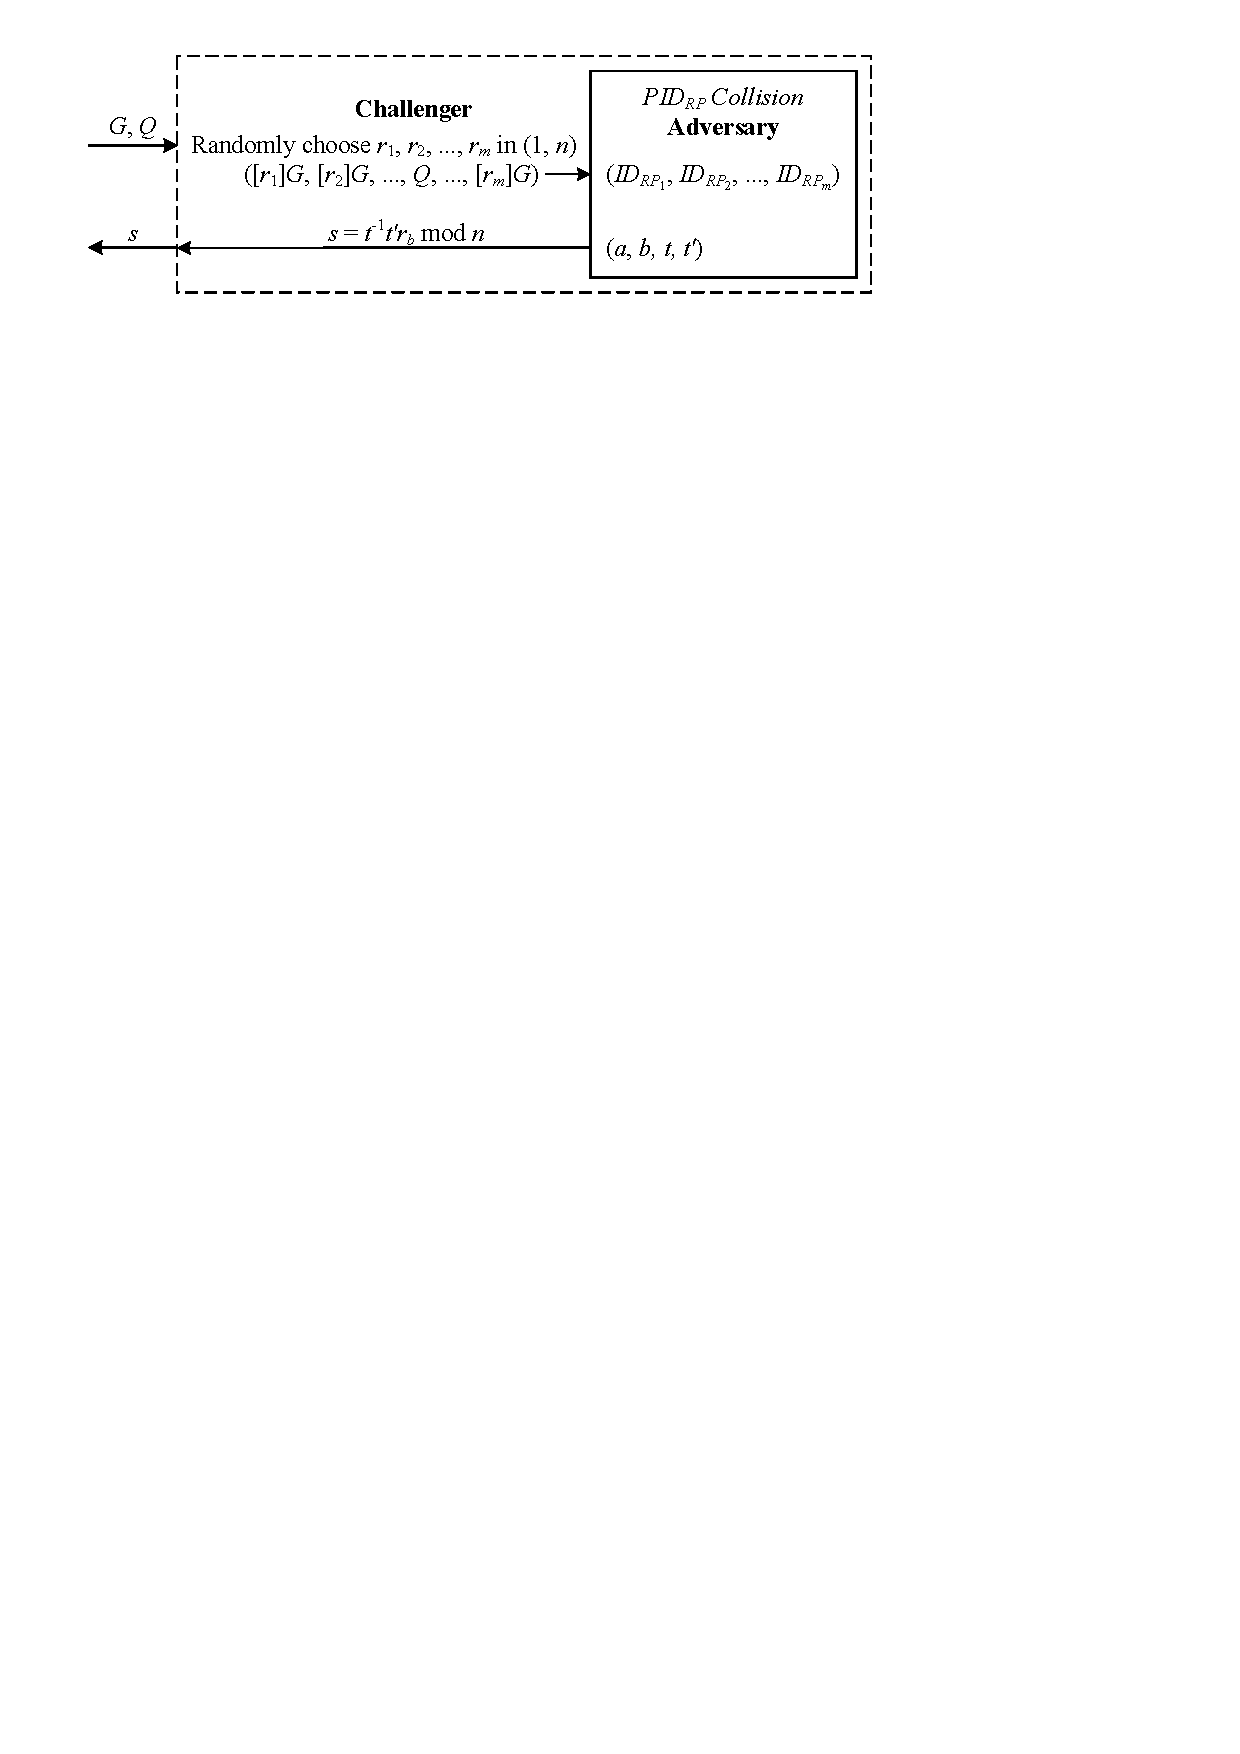
\includegraphics[width=0.96\linewidth]{fig/ecdlp_algorithm.pdf}
  \caption{The PPT algorithm $\mathcal{D}^*_c$ constructed based on the $PID_{RP}$ collision game to solve the ECDLP.}
  \label{fig:ecdlp_algorithm}
\end{figure}

The algorithm $\mathcal{D}^*_c$ works as below.
The input of $\mathcal{D}^*_c$ is in the form of ($G, Q$). On receiving an input ($G$, $Q$), the challenger first randomly chooses $r_1, \cdots, r_m$ in $\mathbb{Z}_n$ to calculate $[r_1]G, \cdots, [r_m]G$.
Then, it randomly chooses $j \in [1,m]$, replaces $[r_j]G$ with $Q$, and sends $m$ RP identities to the adversary, which returns the result ($a$, $b$, $t$, $t'$). Finally, the challenger calculates $s = t^{-1}t'r_b \bmod n$ and returns $s$ as the output of $\mathcal{D}^*_c$.

If the adversary succeeds in $\mathcal{G}_c$ and $[r_a]G$ happens to be replaced with $Q$, then $\mathcal{D}^*_c$ outputs $s=t^{-1}t'r_b =x$ because $[tr_a]G = [t]Q = [t'r_b]G$. For the adversary, $Q$ is indistinguishable from any other RP identities in the input set, as $[r_j]G$ is randomly replaced by the challenger.
Hence, the probability of solving the ECDLP using $\mathcal{D}^*_c$ is formulated as:
\begin{equation*}
{\rm Pr}\{\mathcal{D}^*_c(G, [x]G)=x\} = {\rm Pr}\{s = x\}={\rm Pr}\{a=j\}{\rm Pr}_s=\frac{1}{m}{\rm Pr}_s
\end{equation*}

If the probability of finding $t$ and $t'$ satisfying $[t]ID_{RP_j} = [t']ID_{RP_{j'}}$ is non-negligible, the adversary would have advantages  in $\mathcal{G}_c$ and ${\rm Pr}_s$ is non-negligible regardless of the security parameter $\lambda$.
Thus, we would find that ${\rm Pr}\{\mathcal{D}^*_c(G, [x]G)=x\}$ also becomes non-negligible even when $\lambda$ is sufficiently large, because $m$ is a finite integer and $m \ll 2^\lambda$.
\oldc
This violates the ECDLP assumption. Therefore, the probability of finding $t$ and $t'$ that satisfy $[t]ID_{RP_j} = [t']ID_{RP_{j'}}$ is negligible. \hfill $\square$


\newc

\begin{thm}
\textsc{(User Identification of $TK$)} \emph{$PID_U= [ID_U]PID_{RP}$ in $TK$ uniquely identifies an account at the RP designated by $PID_{RP}$, and this account is uniquely mapped to a user with $ID_U$.}
\label{thm-user-id}
\end{thm}

\noindent\textsc{Proof.}
To issue an identity token requested for $PID_{RP}$, the honest IdP calculates $PID_U = [ID_U]PID_{RP}$ following Equation \ref{equ:PIDU} after authenticating the user with $ID_U$. The designated RP then calculates $Acct = [t^{-1}]PID_{U} = [ID_U]ID_{RP}$ following Equation \ref{equ:AccountNotChanged}.
$Acct = [ID_U]ID_{RP}$ is a \emph{permanent} identifier that is determined once the RP and the user have registered at the IdP. Therefore, $PID_U$ in $TK$ always identifies an account at the designated RP and $Acct$ is mapped to a user with $ID_U$.

Next, we prove that $PID_{U}$ \emph{uniquely} identifies one user in the system and one account at the RP. Since $\mathbb{E}$ is a finite cyclic group, $ID_{RP} = [r]G$ is also a generator on $\mathbb{E}$ of order $n$. Given a user with $ID_U$, $Acct = [ID_U]ID_{RP}$ is a \emph{unique} point on $\mathbb{E}$ for any $u \in [1, n)$, which is \emph{uniquely} associated to $ID_U=u$. \hfill $\square$


\newc

\begin{thm}
\textsc{(Token Integrity)} \emph{An identity token issued by the IdP cannot be forged or manipulated.}
\label{thm-integrity}
\end{thm}


\noindent \textsc{Proof.} Identity tokens are generated and signed by the honest IdP using its private key, which is sufficiently protected at the IdP against adversaries.
%Meanwhile, the IdP's public key $PK$ is sent from the IdP to the RPs.
%and $PK$ which are pre-installed by an RP cannot be manipulated by adversaries.
With the pre-installed public key, an RP verifies the identity tokens it receives and rejects any forged or manipulated identity tokens. Finally, according to the conclusions of the DYU model, the elements in a verified token cannot be manipulated by malicious entities.
\hfill $\square$


\begin{thm}
\textsc{(Token Confidentiality)} \emph{An identity token is accessible only to its designated RP, besides the requesting user and the IdP.}
\label{thm-confidentiality}
\end{thm}

\noindent\textsc{Proof.}
An identity token is generated by the IdP and then sent to the requesting user (i.e., its IdP script).
The IdP script verifies if $ID_{RP}$ specified in a verified RP certificate is designated by $PID_{RP}$ in the identity token and forwards the token to the correct RP script, which is downloaded from the origin of $Enpt_{RP}$ specified also in the RP certificate. %Because the IdP script calculates $PID_{RP} =[t]ID_{RP}$ based on $ID_{RP}$ in this verified RP certificate, this RP is designated in the identity token and will receive the token from the RP script.
As all the communications between the IdP, RPs, and users are protected by HTTPS and two scripts communicate with each other through restricted \verb+postMessage+ HTML5 channels, according to the conclusions of the \dyu\ model, the identity tokens cannot be leaked to any other entities. \hfill $\square$



\begin{thm}
\textsc{(Security)} \emph{\usso\ provides secure authentication services.}
\end{thm}

\noindent\textsc{Proof.}
According to the formal analysis on SSO security \cite{SPRESSO, FettKS14},
    an SSO system satisfying the following two requirements provides \emph{secure} authentication services in the first adversarial scenario: (\emph{a}) an adversary never obtains a valid identity token issued for an honest user and presents it to an honest RP, and (\emph{b}) an honest user never presents a valid identity token that is not issued for herself to an honest RP.

Following the login flow of \usso, because the integrity and confidentiality of identity tokens are satisfied in Theorems \ref{thm-integrity} and \ref{thm-confidentiality},
 no adversary could obtain a valid identity token that is issued to an honest user for accessing an honest RP. %and accepted by an honest RP.
Meanwhile, if an adversary presents an identity token to an honest RP, which may be issued to the adversary for accessing another RP or to an honest user for accessing a colluding RP, RP designation and user identification, proved in Theorems \ref{thm-rp-designation} and \ref{thm-user-id}, ensure that the honest RP does not derive an honest user's account from this identity token.
%Meanwhile, $PID_U$ can only be calculated by the IdP and the user, since no one else knows or could intercept $u$ according to the DYU model. \oldc

According to the login flow and the \dyu\ model, an honest user always obtains identity tokens issued to herself, because $PID_U$ is calculated based on her identity.
  %% which is protected against adversaries. 这一句,对于security没有用,protecting u是用于privacy。
The confidentiality and integrity of identity tokens ensure that an honest user never presents any token issued for someone else to an honest RP. Finally, with user identification,\footnote{\newc RP designation is a precondition of user identification in \usso, but this may not always be necessary for other SSO systems.} her identity tokens are always associated with her account at the target RP.
%According to the conclusions of the DYU model, $PID_U$ is calculated based on the user when the IdP issues an identity token for an authenticated user.
%Moreover, because the confidentiality and integrity of identity tokens are satisfied, an honest user never presents a valid token that is issued to other users.
%When the user identification is satisfied, this token always derives this honest user's account.
%So, an honest user never presents an identity token that is accepted by an honest RP to derive another user’s account at this RP.

Thus, \usso\ is a secure SSO system.
\hfill $\square$

%Finally, according to Theorems 1, 2, 3, 4, and 5, UPPRESSO is secure.

\subsection{Privacy}
\label{sec-:analysis}
\usso\ effectively prevents the privacy threats of IdP-based login tracing and RP-based identity linkage in the second and third adversarial scenarios, respectively.

\newc
First, we show that an honest-but-curious IdP cannot trace a user's login activities. In each login, a user sends an identity-token request to the IdP, %(Step 3.1 in Section \ref{implementations})
which reveals only the target RP's \emph{ephemeral} pseudo-identity $PID_{RP}$ along with the user's identity $ID_U$.
The IdP cannot (\emph{a}) associate multiple logins with different $PID_{RP}$s to a given RP, or (\emph{b}) distinguish a login to one RP from other logins to another RP based on their $PID_{RP}$s, because $PID_{RP}$ is \emph{indistinguishable} from random variables to the IdP.
We prove this in Theorem \ref{thm-idp-untraceability}.

\begin{thm}
\textsc{(IdP Untraceability)} \emph{In \usso, the IdP cannot distinguish $PID_{RP} = [t]ID_{RP}$ from a random variable on $\mathbb{E}$, where $t$ is random in $\mathbb{Z}_n$.}
\label{thm-idp-untraceability}
\end{thm}

\noindent \textsc{Proof.}
Consider a finite cyclic group $\mathbb{E}$ where the number of points on $\mathbb{E}$ is $n$.
Because $G$ is a generator of order $n$, $ID_{RP} = [r]G$ is also a generator on $\mathbb{E}$ of order $n$. According to the \dyu\ model, $t$ is randomly chosen in $\mathbb{Z}_n$ and kept unknown to the IdP. Therefore, $PID_{RP} = [t]ID_{RP}$ is \emph{indistinguishable} from a point $Q$ that is randomly chosen on $\mathbb{E}$ \cite{oprf-proved,voprf-proved,oprf-bitcoin-wallet}.\footnote{\newc This property has been actually proved in OPRFs \cite{oprf-proved,voprf-proved,oprf-bitcoin-wallet}, where the OPRF server works similarly to the IdP and learns \emph{nothing} about a client's inputs or outputs of the evaluated pseudo-random function.} \hfill $\square$


\vspace{2mm}

In the third adversarial scenario, malicious RPs collude with malicious users,
 attempting to link the logins initiated by an honest user but visiting different colluding RPs.
In each login an RP learns an ephemeral identifier $PID_{U} = [{ID_U}]{PID_{RP}}$ and a permanent identifier $Acct = [ID_U]ID_{RP}$ of the user, but it cannot derive $ID_U$ from $PID_{U}$ or $Acct$ due to the ECDLP.
Therefore, the colluding adversaries share all logins to malicious RPs,
    and attempt to leverage the logins initiated by malicious users to link the other logins by honest users.


In \usso, an RP receives a random number $t$ and an identity token enclosing $PID_{RP}$ and $PID_U$ in each login. %Meanwhile, it knows its own identity $ID_{RP}$, from which it also derives the user's account $Acct$.
With the trapdoor $t$, $PID_{RP}$ and $PID_U$ can be easily transformed into $ID_{RP}$ and $Acct$, respectively, and vice versa. Therefore, we denote the information that an RP learns from a login as a tuple $L$, where $L =(ID_{RP}, t, Acct)=(ID_{RP}, t, [ID_{U}]ID_{RP})=([r]G, t, [ur]G)$.


%Hence, an $RP_j$ with $w$ logins knows $\{L_{1,j},...,L_{w,j}\}$.

When $c$ malicious RPs collude with each other, they create a shared view of all their logins, denoted as $\mathbb{L}$.
%some of which are initiated by honest users and denoted as $\mathbb{L}^h$, and the others by $v$ malicious users  are $\mathbb{L}^m = \mathbb{L} \setminus \mathbb{L}^h$.
When they collude further with $v$ malicious users, the logins initiated by these malicious users are picked out and linked together as
$\mathfrak{L}^m=\left \{ \begin{matrix}
L^m_{1,1},&L^m_{1,2},&\cdots,&L^m_{1,c}\\
L^m_{2,1},& L^m_{2,2},&\cdots,&L^m_{2,c}\\
\cdots,&\cdots,&L^m_{i,j},&\cdots\\
L^m_{v,1},&L^m_{v,2},&\cdots,&L^m_{v,c}
\end{matrix}\right\}$,
where $L^m_{i, j}=([r_j]G, t_{i,j}, [u_ir_j]G)$ for $1 \le i \le v$ and $1 \le j \le c$, and $L^m_{i,j} \in \mathbb{L}$. Any login in $\mathbb{L}$ but not linked in $\mathfrak{L}^m$ is initiated by an honest user to one of the $c$ malicious RPs.


\begin{thm}
\textsc{(RP Unlinkability)} \emph{In \usso, given $\mathbb{L}$ and $\mathfrak{L}^m$, $c$ malicious RPs and $v$ malicious users cannot link any login visiting a malicious RP by an honest user to any subset of logins visiting any other malicious RPs by honest users.}
\end{thm}


\noindent\textsc{Proof.} From the logins in $\mathbb{L}$,
 we randomly choose one login $L' \neq L^m_{i,j}$,
 which is from an (unknown) honest user with $ID_{U'}=u'$ to a malicious $RP_a$ and $a \in [1,c]$.
Then, we randomly choose another malicious $RP_b$, where $b \in [1,c]$ and $b \neq a$.
Consider any subset $\mathbb{L}''$ of $w$ logins visiting $RP_b$ by unknown honest users,
 we denote the identities of the honest users who initiate these logins as $\mathbf{u}_w=\{{u''_1}, {u''_2}, \cdots, {u''_w}\}$.
Next, we prove that the colluding adversaries cannot decide if $u'$ is in $\mathbf{u}_w$ or randomly selected from the universal user set.
This indicates the colluding adversaries cannot link $L'$ to another login visiting $RP_b$
    or to another subset of logins visiting $RP_b$.

We first define an RP-based linkage game $\mathcal{G}_r$ between an adversary and a challenger, which describes this login linkage privacy threat: the adversary receives $\mathfrak{L}^m$, $L'$, and $\mathbb{L}''$ from the challenger and outputs $s$, where $s = 1$ if it decides $u'$ is in $\mathbf{u}_w$ %$\{{U''_1}, {U''_2}, \cdots, {U''_w}\}$
and $s=0$ if it believes $u'$ is randomly chosen from the universal user set.
Thus, the adversary succeeds in $\mathcal{G}_r$ with an advantage $\mathbf{Adv}_{A}$:
\begin{align*}
%&{\rm Pr}_1={\rm Pr}\{\mathcal{G}_r(\mathfrak{L}, L', \mathbb{L}'' | u' \in \{{u''_1}, {u''_2}, \cdots, {u''_w}\})=1\} \\
&{\rm Pr}_1={\rm Pr}(\mathcal{G}_r(\mathfrak{L}^m, L', \mathbb{L}'')=1 \;| \; u' \in \mathbf{u}_w)  \\
%&{\rm Pr}_2={\rm Pr}\{\mathcal{G}_r(\mathfrak{L}, L', \mathbb{L}'' | u' \in \mathbb{Z}_n)=1\}\\
&{\rm Pr}_2={\rm Pr}(\mathcal{G}_r(\mathfrak{L}^m, L', \mathbb{L}'')=1 \; | \; u' \in \mathbb{Z}_n)\\
&{\mathbf{Adv}}_{A}=|{\rm Pr}_1-{\rm Pr}_2|
\end{align*}

As depicted in Figure \ref{fig:dalgorithm}, we design a PPT algorithm $\mathcal{D}^*_r$ based on $\mathcal{G}_r$ to solve the elliptic curve decisional Diffie-Hellman (ECDDH) problem: given $(G, [x]G$, $[y]G$, $[z]G)$, decide whether $z$ is equal to $xy$ or randomly chosen in $\mathbb{Z}_n$, where $G$ is a point on an elliptic curve $\mathbb{E}$ of order $n$, and $x$ and $y$ are integers randomly and independently chosen in $\mathbb{Z}_n$.


\begin{figure}[tb]
  \centering
  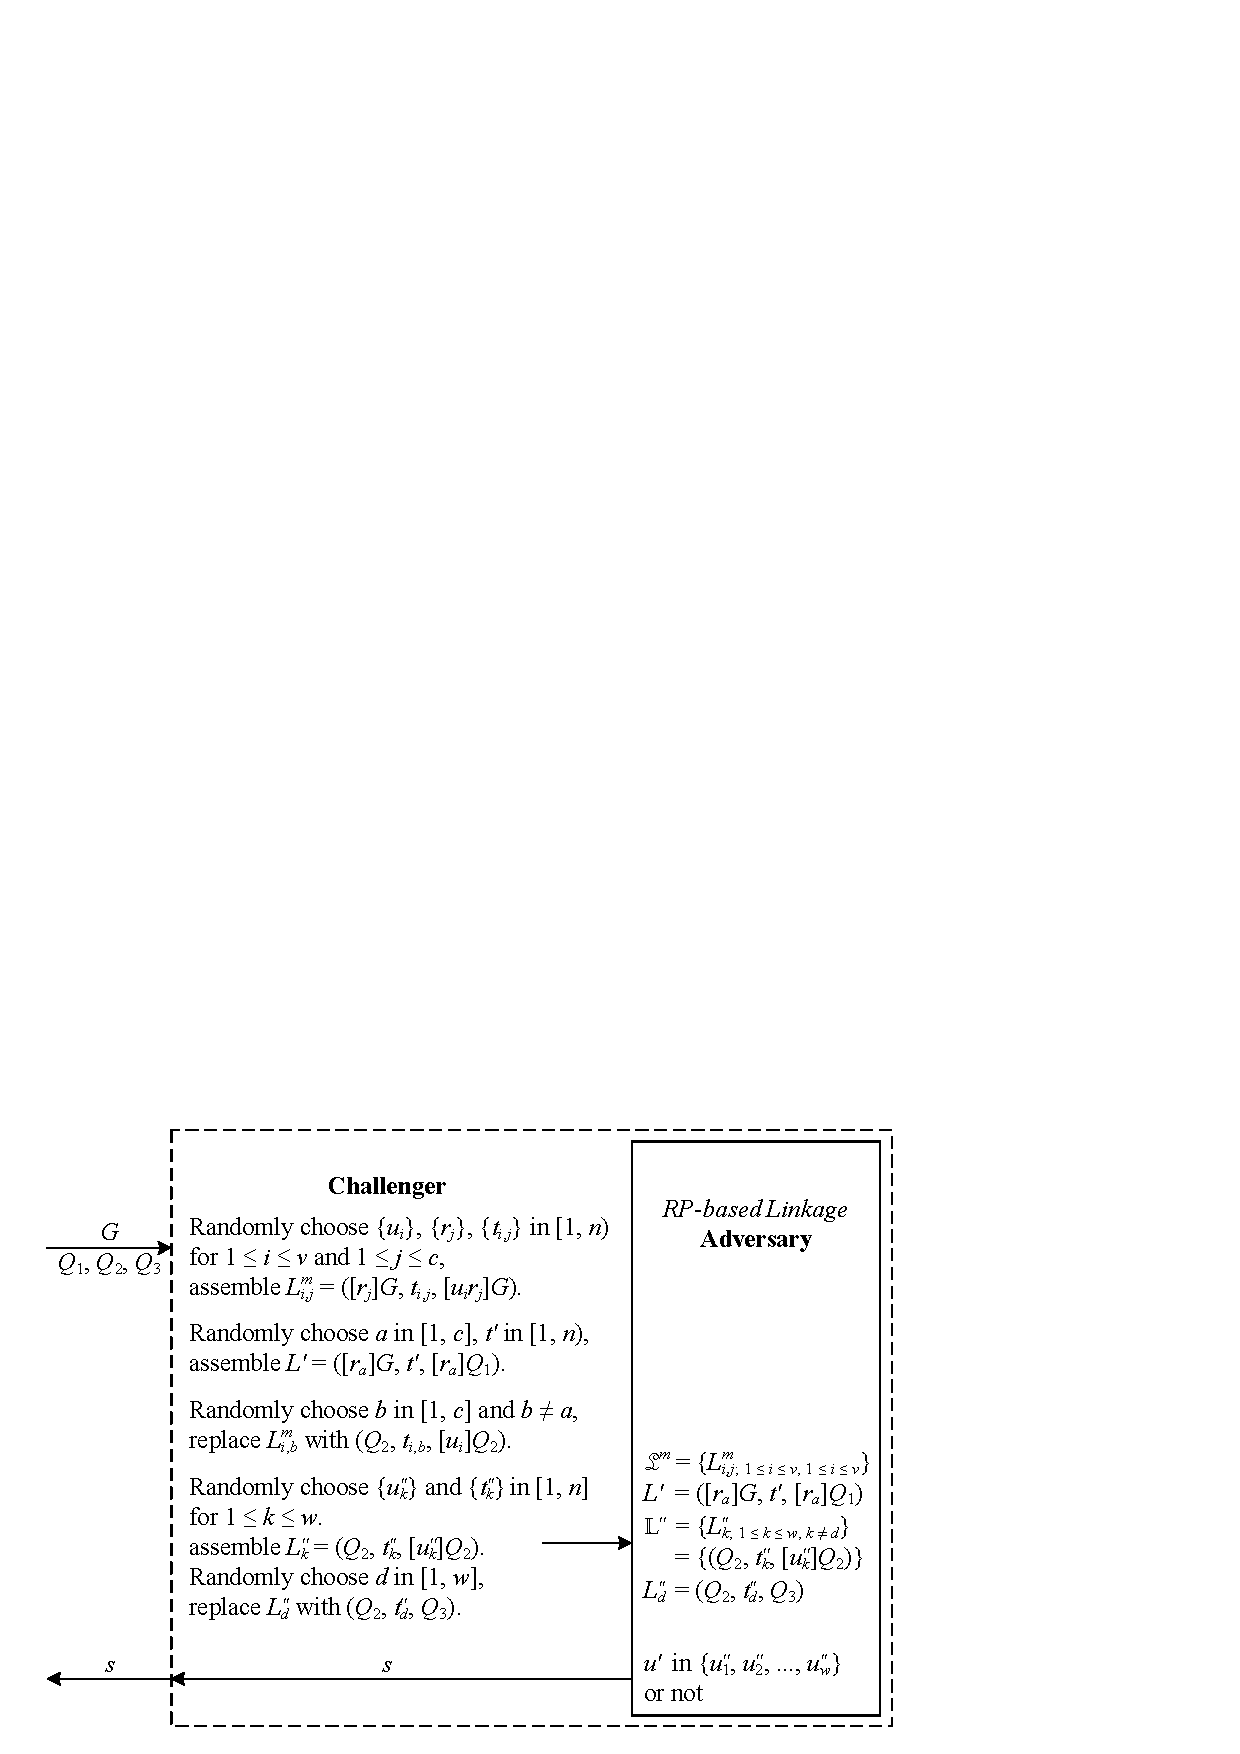
\includegraphics[width=1.0\linewidth]{fig/rp-linkage-game.pdf}
  \caption{The PPT algorithm $\mathcal{D}^*_r$ constructed based on the RP-based linkage game to solve the ECDDH problem.}
  \label{fig:dalgorithm}
\end{figure}


The algorithm $\mathcal{D}^*_r$ works as below. (1) Upon receiving an input $(G, Q_1=[x]G, Q_2=[y]G, Q_3=[z]G)$, %of $\mathcal{D}^*_r$
the challenger
chooses random numbers in $\mathbb{Z}_n$ to construct $\{u_i\}$, $\{r_j\}$, and $\{t_{i, j}\}$ for $1 \le i \le v$ and $1 \le j \le c$, with which it assembles $L^m_{i, j}=([r_j]G, t_{i,j}, [u_ir_j]G)$.
In this process, it ensures $[r_{j}]G \neq Q_2$ so that $r_j \neq y$.  % 这个应该反过来讲;因为y是离散对数。
(2) It randomly chooses $a \in [1, c]$ and $t' \in \mathbb{Z}_n$, to assemble $L' = ([r_{a}]G, t', [r_{a}]Q_1) = ([r_{a}]G, t', [xr_{a}]G)$.
(3)
% Here, $L'$ represents the knowledge of the login visiting $RP_{j'}$ by a user with $ID_U = x$.
Next, the challenger randomly chooses $b \in [1, c]$ and $b \neq a$, and replaces $ID_{RP_b}$ with $Q_2 = [y]G$.
Hence, for $1 \le i \le v$, the challenger replaces $L^m_{i, b}=([r_b]G, t_{i,b}, [u_ir_b]G)$ with $(Q_2, t_{i,b}, [u_i]Q_2) = ([y]G, t_{i,b}, [u_iy]G)$, and then constructs $\mathfrak{L}^m$.
(4) the challenger chooses random numbers in $\mathbb{Z}_n$ to construct $\{u''_k\}$ and $\{t''_k\}$ for $1 \leq k \leq w$,
 with which it assembles $\mathbb{L}'' = \{L''_{k; 1\leq k \leq w}\} = \{(Q_2, t''_k, [u''_k]Q_2)\} = \{([y]G, t''_k, [u''_ky]G)\}$.
In this process, it ensures that $[u''_k]G \neq Q_1$ (i.e., $u''_k \neq x$) and $u''_k \neq u_i$,
 for $1 \le i \le v$ and $1 \le k \le w$.
Finally, it randomly chooses $d \in [1, w]$ and replaces $L''_{d}$ with $(Q_2, t''_d, Q_3) = ([y]G, t''_d, [z]G)$.
 Thus, $\mathbb{L}'' = \{L''_{k;1\leq k \leq w}\}$ represents the logins from $w$ honest users, i.e., $\mathbf{u}_w=\{u''_1, u''_2, \cdots, u''_{d-1}, z/y, u''_{d+1}, \cdots, u''_w\}$. (5) When the adversary receives $\mathfrak{L}^m$, $L'$, and $\mathbb{L}''$ from the challenger, it returns $s$ as the output of $\mathcal{D}^*_r$.

According to the above construction, % of $\mathfrak{L}$, $L'$ and $\mathbb{L}''$,
$x$ is embedded as $ID_{U'}$ in the login $L'$ visiting the RP with $ID_{RP_{a}} = [r_{a}]G$,
and $z/y$ is embedded as $ID_{U''_d}$ in $\mathbb{L}''$ visiting the RP with $ID_{RP_{b}}=[y]G$,
together with $\{u''_1, \cdots, u''_{d-1}, u''_{d+1}, \cdots, u''_w\}$.
Meanwhile, $[r_{a}]G$ and $[y]G$ represent two malicious RPs in $\mathfrak{L}^m$.
Because $x$ is not in $\{u''_1, \cdots, u''_{d-1}, u''_{d+1}, \cdots, u''_w\}$, i.e., $x \neq u''_{k; 1\leq k \leq w, k \neq d}$, the adversary outputs $s=1$ and succeeds in the game \emph{only if} $x = z/y$.
% 这里不是if and only if. "if, 就变成了the adversary必胜了;并不是,而是“有显著的概率”"
% 当“the adversary outputs s=1 且 succeeds in the game”,=> "x = z/y"
% 但是,"x = z/y"  => 不能推导得到“the adversary outputs s=1 且 succeeds in the game”。因为adversary有时候fail、不总是succeed
 Therefore, using $\mathcal{D}^*_r$ to solve the ECDDH problem, we have an advantage $\mathbf{Adv}^*_{A}=|{\rm Pr}^*_1 - {\rm Pr}^*_2|$, where
\begin{align*}
&{\rm Pr}^*_1 =  {\rm Pr}(\mathcal{D}^*_r(G, [x]G, [y]G, [xy]G)=1) \\
=&{\rm Pr}(\mathcal{G}_r(\mathfrak{L}^m, L', \mathbb{L}'')=1 \; | \; u' \in \mathbf{u}_w) = {\rm Pr}_1 \\
&{\rm Pr}^*_2= {\rm Pr}(\mathcal{D}^*_r(G, [x]G, [y]G, [z]G)=1) \\
=&{\rm Pr}(\mathcal{G}_r(\mathfrak{L}^m, L', \mathbb{L}'')=1 \; | \; u' \in \mathbb{Z}_n) = {\rm Pr}_2 \\
&\mathbf{Adv}^*_{A}=|{\rm Pr}^*_1-{\rm Pr}^*_2|=|{\rm Pr}_1-{\rm Pr}_2|={\mathbf{Adv}}_{A}
\end{align*}

If the adversary has a non-negligible advantage in $\mathcal{G}_r$, then $\mathbf{Adv}^*_{A}={\mathbf{Adv}}_{A}$ is also non-negligible regardless of the security parameter $\lambda$. This violates the ECDDH assumption. Therefore, the adversary has no advantage in $\mathcal{G}_r$ and cannot decide whether $L'$ is initiated by some user with an identity in $\mathbf{u}_w$ or by a user in the universal user set.
Moreover, because $RP_b$ is any malicious RP, this proof can be easily extended from $RP_b$ to more colluding malicious RPs.
\hfill $\square$

\oldc

